%%%%%%%%%%%%%%%%%%%%%%%%%%%%%%%%%%%%%%%%%%%%%%%%%%%%%%%
% MatPlotLib and Random Cheat Sheet
%
% Edited by Michelle Cristina de Sousa Baltazar
%
% http://matplotlib.org/api/pyplot_summary.html
% http://matplotlib.org/users/pyplot_tutorial.html
%
%%%%%%%%%%%%%%%%%%%%%%%%%%%%%%%%%%%%%%%%%%%%%%%%%%%%%%%

\documentclass{article}
\usepackage[landscape]{geometry}
\usepackage{url}
\usepackage{multicol}
\usepackage{amsmath}
\usepackage{amsfonts}
\usepackage{tikz}
\usetikzlibrary{decorations.pathmorphing}
\usepackage{amsmath,amssymb}
\usepackage{wrapfig}
\usepackage{colortbl}
\usepackage{amsfonts}       % blackboard math symbols
\usepackage{amsmath}
\usepackage{amssymb}
\usepackage{graphicx}
\usepackage{csquotes}
\usepackage[backend=biber, style=apa,]{biblatex}
\usepackage{setspace}
% \usepackage[usenames, dvipsnames]{xcolor}
% Define Verilog style
\usepackage{listings}
\lstdefinelanguage{riscv}{
  morekeywords={add,sub,mul,div,addi,subi,lw,sw,beq,bne,jal,jalr,jr,li,and,andi,j,la,bnez,beqz},
  sensitive=false,
  morecomment=[l]{\#},
  morestring=[b]",
}
\lstdefinelanguage{do}{
  morekeywords={force, run, log, vsim, vlib, vlog},
  sensitive=false,
  morecomment=[l]{\#},
  morestring=[b]",
}
\lstdefinestyle{verilogStyle}{
    language=Verilog,
    basicstyle=\tiny\ttfamily,
    keywordstyle=\color{black},
    commentstyle=\color{black},
    stringstyle=\color{black},
    showstringspaces=false,
    frame=single,
    breaklines=true,
    breakatwhitespace=true,
    tabsize=2,
    captionpos=b,
    xleftmargin=0pt
}
\lstdefinestyle{doStyle}{
    language=do,
    basicstyle=\tiny\ttfamily,
    keywordstyle=\color{black},
    commentstyle=\color{black},
    stringstyle=\color{black},
    showstringspaces=false,
    frame=single,
    breaklines=true,
    breakatwhitespace=true,
    tabsize=2,
    captionpos=b,
    xleftmargin=0pt
}
\lstdefinestyle{assembly}{
    language=riscv,
    basicstyle=\tiny\ttfamily,
    keywordstyle=\color{black},
    commentstyle=\color{black},
    stringstyle=\color{black},
    showstringspaces=false,
    frame=single,
    breaklines=true,
    breakatwhitespace=true,
    tabsize=2,
    captionpos=b,
    xleftmargin=0pt
}
\lstdefinestyle{verilogStyle2}{
    language=Verilog,
    basicstyle=\tiny\ttfamily,
    keywordstyle=\color{black},
    commentstyle=\color{black},
    stringstyle=\color{black},
    showstringspaces=false,
    frame=single,
    breaklines=true,
    breakatwhitespace=true,
    tabsize=2,
    captionpos=b,
    xleftmargin=0pt
}

% Set default style to Verilog
\lstset{style=verilogStyle}
\usepackage{caption}
\usepackage{subcaption}
\usepackage{multirow}
\usepackage{float}
\usepackage{wrapfig}
\usepackage{placeins}
\usepackage{algpseudocode}

\usepackage{algorithm}
\usepackage{algorithmicx}
\usepackage{hyperref}
\usepackage{mathtools}
\usepackage{amsmath,amssymb}
\usepackage{enumitem}

\title{MatPlotLib and Random Cheat Sheet}
\usepackage[brazilian]{babel}
\usepackage[utf8]{inputenc}
\newcommand{\topscore}{Top$^{\text{score}}$}
\advance\topmargin-.8in
\advance\textheight3in
\advance\textwidth3in
\advance\oddsidemargin-1.5in
\advance\evensidemargin-1.5in
\parindent0pt
\parskip2pt
\newcommand{\hr}{\centerline{\rule{3.5in}{1pt}}}
%\colorbox[HTML]{e4e4e4}{\makebox[\textwidth-2\fboxsep][l]{texto}
\begin{document}

% \begin{center}{\huge{\textbf{MatplotLib and Random Cheat Sheet}}}\\
% {\large By Michelle Cristina de Sousa Baltazar}
% \end{center}
\begin{multicols*}{3}

\tikzstyle{mybox} = [draw=black, fill=white, very thick,
    rectangle, rounded corners, inner sep=10pt, inner ysep=10pt]
\tikzstyle{fancytitle} =[fill=black, text=white, font=\bfseries]
%------------ CONTEÚDO CAIXA RANDOM ---------------
\begin{tikzpicture}
\node [mybox] (box){%
    \footnotesize\begin{minipage}{0.3\textwidth}
        \textbf{MinTerms}: Corresponds to SOP, ecaluates to 1. i.e.  $m_{0,0,1}|_{f=1}=\Bar{x_1}\Bar{x_2}x_3,\;SOP=\sum_{ijk}m_{ijk}$\\
        \textbf{MinTerms}: Corresponds to POS, ecaluates to 0. i.e. $M_{0,1,1}|_{f=0}=x_1+\Bar{x_2}+\Bar{x_3},\;POS=\prod_{ijk}M_{ijk}$\\
        % \textbf{Karnaugh Map}: Minterms version: ($\Bar{x_2}\Bar{x_4}+x_2x_1+\Bar{x_4}x_2$)
        % \begin{center}
        %     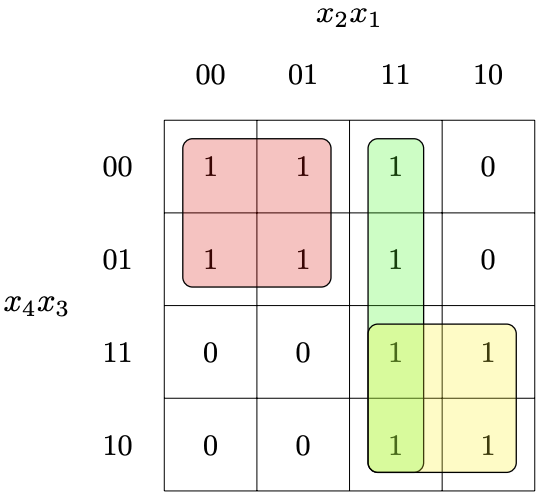
\includegraphics[width=0.35\columnwidth]{k.png}
        % \end{center}
        \textbf{2's Complement} Given a number $+k$ in $n$ bits, we compute $-k$ as $2^n-k$. Shortcut: complement every bit and add 1\\
        \textbf{Tristate Buffer}: Control signal $e$, if high, high impedance
    \end{minipage}
};
%------------ CAIXA RANDOM ---------------------
\node[fancytitle, right=10pt] at (box.north west) {Fundamentals};
\end{tikzpicture}


%------------ CONTEÚDO CAIXA MatPlotLib ---------------
\begin{tikzpicture}
\node [mybox] (box){%
    \footnotesize\begin{minipage}{0.3\textwidth}
        \begin{enumerate}[left=3pt, topsep=0pt, partopsep=0pt, parsep=0pt, itemsep=0pt]
            \item $\textbf{mx2}(s,x_0,x_1)=\Bar{s}x_0+sx_1$
            \item $\textbf{mx4}(s_i,x_i)=\textbf{mx2}(\textbf{mx2}(s_0,x_0,x_1),\textbf{mx2}(s_1,x_2,x_3))$
            \item $\textbf{not}(x)=\textbf{nand}(x,x)=\textbf{nor}(x,x)$
            \item $\&=\textbf{mx}(x,y,1),|=\textbf{mx}(x,0,y)\text{ mux functionally complete}$ 
            \item $xy+yz+\Bar{x}z=xy+\Bar{x}z,\;(x+y)(\Bar{x}+z)(y+z)=(x+y)(\Bar{x}+z)$
        \end{enumerate}
    \end{minipage}
};
%------------ CAIXA PRELIMINARES ---------------------
\node[fancytitle, right=10pt] at (box.north west) {Common Logic expressions};
\end{tikzpicture}
%------------ CONTEUDO EXEMPLO BASICO ---------------------
\begin{tikzpicture}
\node [mybox] (box){%
    \footnotesize\begin{minipage}{0.3\textwidth}
        \textbf{RS Latch}
        \vspace{-5pt}
        \begin{center}
            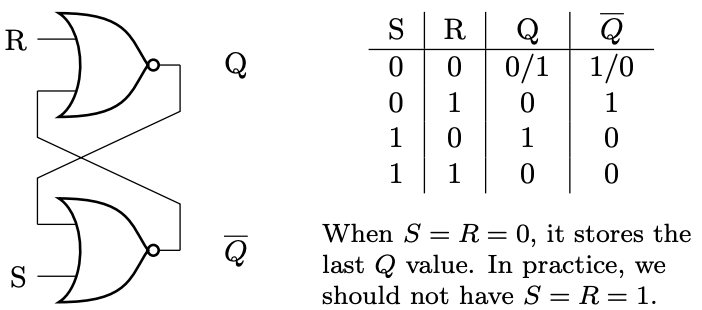
\includegraphics[width=0.6\columnwidth]{rs.png}
        \end{center}
        \textbf{Gated D-Latch}
        \vspace{-5pt}
        \begin{center}
            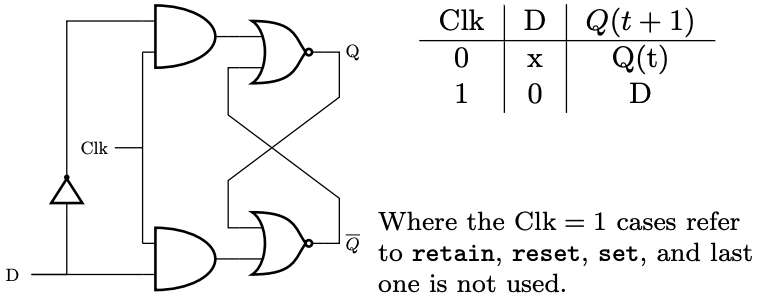
\includegraphics[width=0.72\columnwidth]{gatedd.png}
        \end{center}
        \textbf{D-FF}: 2 GDLs in series, $Q_0-D_1$, with $clk_0=\Bar{clk_0}$
        \vspace{-5pt}
        \begin{center}
            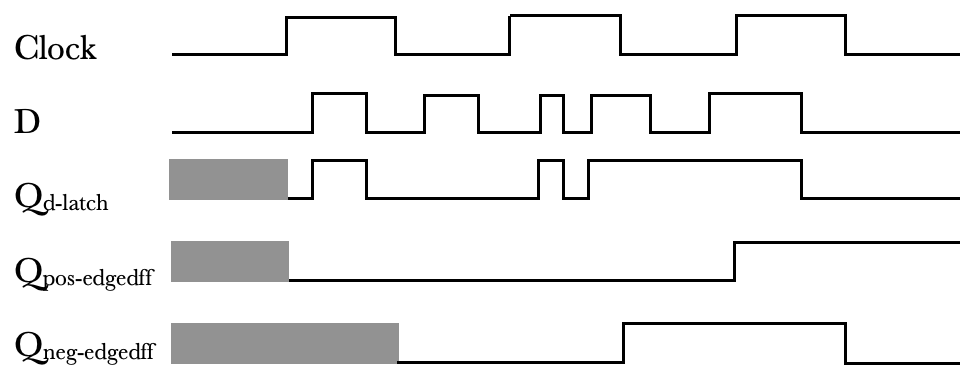
\includegraphics[width=0.7\columnwidth]{time.png}
        \end{center}
        \textbf{Resets}: Synchronous (SR) resets the next posedge clk, asynchronous (AR) resets as soon as resetn low\\
        \textbf{Enables}: If $e=0$, $D=Q$, else it is a normal flipflop\\
        \textbf{T-FF}: DFF with $D=T\text{\textasciicircum}Q$. To build counting circuit, use AR T-FFs connected via $T_0=1,T_1=Q_0\cdot1,T_2=Q_0\cdot Q_1, T_n=Q_{n-2}\cdot Q_{n-1}$. $Q_{t+1}=Q(t)\text{\textasciicircum}T$
        \vspace{-5pt}
        \begin{center}
            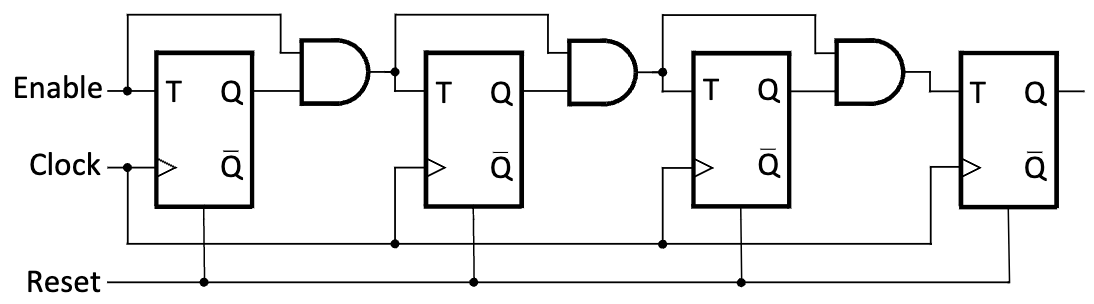
\includegraphics[width=0.9\columnwidth]{count.png}
        \end{center}
        \vspace{-10pt}
    \end{minipage}
};
%------------ EXEMPLO BASICO BOX ---------------------
\node[fancytitle, right=10pt] at (box.north west) {Combinational Logic};
\end{tikzpicture}
%------------ CONTEUDO DOIS EIXOS ---------------------
\begin{tikzpicture}
\node [mybox] (box){%
    \begin{minipage}{0.3\textwidth}
    \setstretch{0.9}
\begin{lstlisting}
module FA(input logic a, b, cin, output logic s, cout);
    assign s=a^b^c;
    assign cout=(a&b)|(cin&a)|(cin&b);
endmodule

module adder3(input logic [2:0] A, B, input logic cin, output logic [2:0] s, output logic cout);
    logic c1, c2;
    FA u0(A[0], B[0], c_in, s[0], c1);
    FA u1(A[1], B[1], c_1, s[0], c2);
    FA u2(A[1], B[2], c_2, s[0], cout);
endmodule

module D_latch(input logic D, clk, output logic Q);
    always_latch
        if (clk) Q=D;
endmodule

module reg8(input logic [7:0] D, input logic clk, output logic [7:0] Q); // for D_FF same w/o bus
    always_ff @(posedge clk)
        Q<=D;
endmodule

module D_FFR_sync(input logic D, clk, resetn, output logic Q);
    always_ff @(posedge clk) 
    // for async, add negedge resetn into ff arg
        if (!resetn) Q<=1'b0;
        else Q<=D;
endmodule

module opcount(input logic [3:0] R, input logic resetn, clk, enable, load, output logic [3:0] Q);
    always_ff @(posedge clk, negedge resetn) begin
        if (!resetn) Q<=4'b0;
        elseif (load) Q<=R;
        elseif (enable) Q<=Q+1;
    end
endmodule

module ALU(A, B, Function, ALUout);
    parameter N = 4;
    input logic [N-1:0] A, B;
    input logic [1:0] Function;
    output logic [2*N-1:0] ALUout;
    always_comb begin
        case(Function)
        2'b00: ALUout = {N{1'b0}} + A + B;
        2'b01: ALUout = |{A, B};
        2'b10: ALUout = &{A, B};
        2'b11: ALUout = {A, B}; //concat 
        default: ALUout = {(2*N){1'b0}};
        endcase end
endmodule

module FSM(input logic w, clk, resetn, output logic z);
    typedef enum logic [1:0] [A,B,C,D] statetype;
    statetype ps, ns;
    always_ff @(posedge clk, negedge resetn) begin
        if (!resetn) ps<=A;
        else ps<=ns; 
    end 
    always_comb
        case(ps)
        A: if (w) ns=B; else ns=A;
        B: if (w) ns=B; else ns=C; //...
        endcase
    assign z=(ps==D)
endmodule

module FSM_shift_R(input logic w, clock, resetn, output logic z);
    logic [3:1]y;
    always_ff @(posedge clock, negedge resetn)
    begin 
    if (!resetn) y<=3'b000;
    else begin
        y[3]<=w;
        y[2]<=y[3];
        y[1]<=y[2];
    end end
    assign z=y[3]&~y[2]&y[1]
endmodule

module countingCircuit (input logic Clock, logic Enable, Reset, output logic [7:0] CounterValue);
    logic [7:0] b;
    T_flip_flop T7(Clock, Reset, b[6], CounterValue[7], b[7]);
    //...
    T_flip_flop T1(Clock, Reset, b[0], CounterValue[1], b[1]);
    T_flip_flop T0(Clock, Reset, Enable, CounterValue[0], b[0]);
endmodule

module T_flip_flop(input logic clk, reset_b, t, output logic q, t);
    logic d;
    assign d = q ^ t;
    assign b = q & t;
    D_flip_flop dff(.clk(clk), .reset_b(reset_b), .d(d), .q(q));
endmodule
\end{lstlisting}
\vspace{-10pt}
    \end{minipage}
};
%------------ DOIS EIXOS BOX ---------------------
\node[fancytitle, right=10pt] at (box.north west) {Select Verilog Code};
\end{tikzpicture}





%------------ CONTEÚDO COMANDOS DE TEXTO ---------------------
\begin{tikzpicture}
\node [mybox] (box){%
    \footnotesize\begin{minipage}{0.3\textwidth}
    e.g. Goal: return when w has had a sequence of 1, 0 ,1
    \vspace{-5pt}
    \begin{center}
    \footnotesize\begin{tabular}{c|cc|c}
        \centering
        present$(y_2y_1)$ & $w=0(Y_2Y_1)$ & $w=1$ & $z$ \\
        \hline
        $A(00)$& $A(00)$& $B(01)$&0  \\
        $B(01)$& $C(10)$& $B(01)$&0  \\
        $C(10)$& $A(01)$& $D(11)$&0  \\
        $D(11)$& $C(10)$& $B(01)$&1  \\
    \end{tabular}
    \\Using Karnaugh maps, $Y_1=w,\;Y_2=\Bar{w}y_1+wy_2\Bar{y_1},z=y_2y_1$\\
    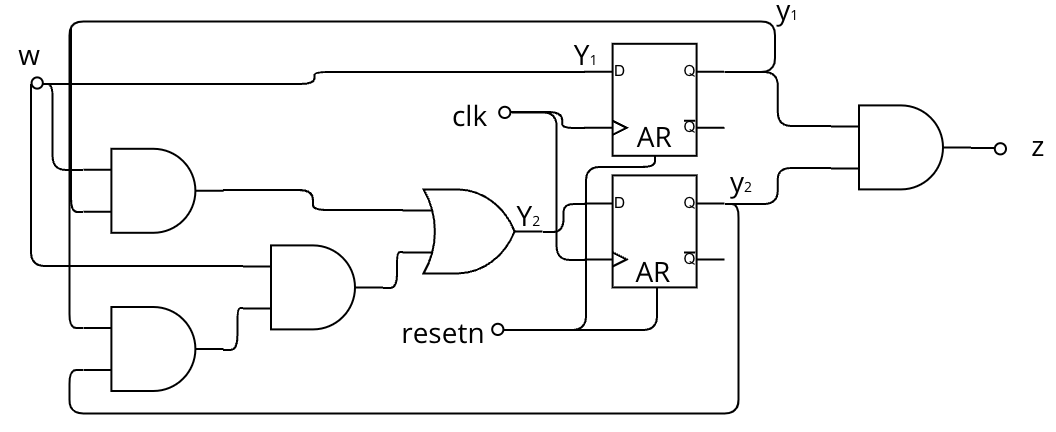
\includegraphics[width=0.9\columnwidth]{fsm.png}
    \end{center}
    \vspace{-10pt}
    Alternatively, make a state diagram in which each state represents last 3 values of $w$. With synthesis, we find that $Y_3=w,Y_1=y_2,Y_2=y_3,z=y_3\Bar{y_2}y_1$\\
    \vspace{-10pt}
    \begin{center}
    \footnotesize\begin{tabular}{c|cc|c}
        \centering
        present($y_3y_2y_1$)& $w=0(Y_3Y_2Y_1)$ & $w=1$ & $z$ \\
        \hline
        $s_{000}$& $000$& $100$&0  \\
        $s_{001}$& $000$& $100$&0  \\
        $s_{010}$& $001$& $101$&0  \\
        $s_{011}$& $001$& $101$&0  \\
        $s_{100}$& $010$& $110$&0  \\
        $s_{100}$& $010$& $110$&1  \\
        $s_{110}$& $011$& $111$&0  \\
        $s_{111}$& $011$& $111$&0  \\
    \end{tabular}
    \end{center}
    \vspace{-10pt}
    \textbf{Shift Register}: Connections of FF in series (refer to verilog)\\
    \vspace{-8pt}
    \centering
    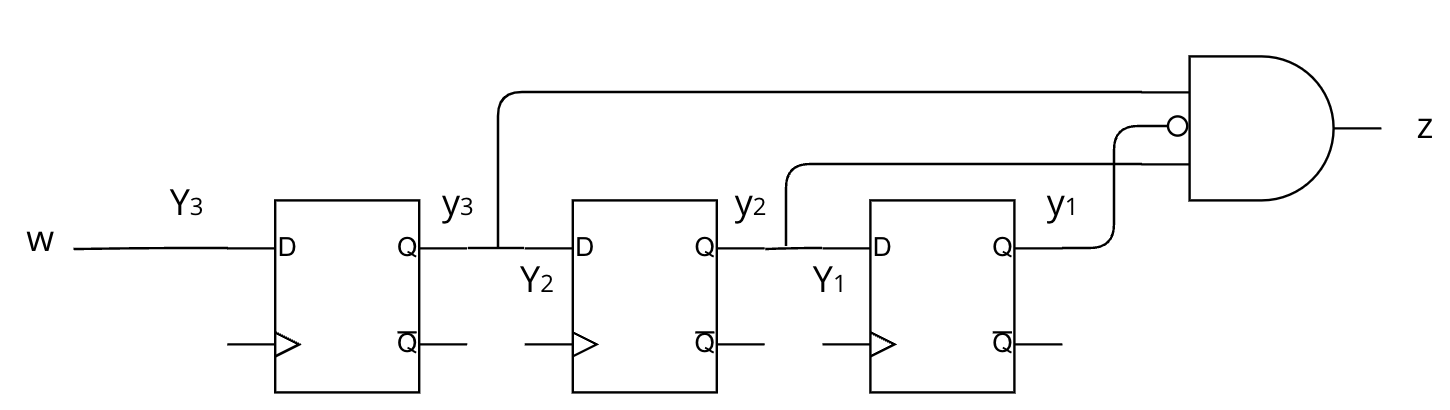
\includegraphics[width=0.8\columnwidth]{sr.png}
    \end{minipage}
};
%------------ COMANDOS DE TEXTO BOX ---------------------
\node[fancytitle, right=10pt] at (box.north west) {Finite State Machines};
\end{tikzpicture}










%------------ CONTEÚDO COMANDOS DE TEXTO ---------------------
\begin{tikzpicture}
\node [mybox] (box){%
    \footnotesize\begin{minipage}{0.3\textwidth}
    \begin{enumerate}[left=3pt, topsep=0pt, partopsep=0pt, parsep=0pt, itemsep=0pt]
        \item Find longest path. \textbf{$T_{su}$, $T_{hold}$}: data D must be stable. $t_{su}$: b/w D posedge and clk posedge; $t_{h}$: b/w clk posedge and D negedge, $T_{min}\geq t_{cQ}+t_{gates,i}+t_{su},F_{max}\leq\frac{1}{T_{min}}$
        \item Consider clock skew. Positive skew ($\Delta>0$, src clk faster than sink clk) allows more time (higher $F_{max}$), negative results in opposite, $T_{min}+\Delta\geq t_{cQ} + t_{gates,i}+t_{su}$
        \item Calculate hold time violation: shortest path b/w 2 FFs, data racing the clk ($t_{su}$ not used). This is $t_{logic-min}$
        \item Setup time violation: logic too slow for correct value to arrive at input to FF by $t_{su}$ before clock edge
        \item Preventing hold time violations: $t_h+\Delta\leq t_{cQ}+t_{logic-min}$
    \end{enumerate}
    \end{minipage}
};
%------------ COMANDOS DE TEXTO BOX ---------------------
\node[fancytitle, right=10pt] at (box.north west) {Timing Analysis};
\end{tikzpicture}



%------------ CONTEÚDO COMANDOS DE TEXTO ---------------------
\begin{tikzpicture}
\node [mybox] (box){%
    \footnotesize\begin{minipage}{0.3\textwidth}
    \lstset{style=dostyle}
    \vspace{-5pt}
    \begin{lstlisting}
vlib work
vlog mux.sv
vsim mux
log {/*} # log all signals 
add wave {/*} # add all items in top level simulation module
force {SW[0]} 0 # single force
force {SW[0]} 0, 1 {10 ns} -r {20 ns} # looped force
force {b} 0 {0ns} , 1 {2ns} -r {5ns} # 0011100111 waveform
run 25ns
    \end{lstlisting}
    \vspace{-10pt}
    \end{minipage}
};
%------------ COMANDOS DE TEXTO BOX ---------------------
\node[fancytitle, right=10pt] at (box.north west) {Modelsim};
\end{tikzpicture}












\newpage
%------------ CONTEUDO PROPRIEDADES ---------------------
\begin{tikzpicture}
\node [mybox] (box){%
    \tiny\begin{minipage}{0.3\textwidth}
    \lstset{style=verilogStyle2}
    \vspace{-7pt}
\begin{lstlisting}
module rotatingRegister(input logic clock, reset, ParallelLoadn, RotateRight, ASRight, input logic [3:0] Data_IN, output logic [3:0] Q);
	logic left_for_ff3;
	assign left_for_ff3 = ASRight ? Q[3] : Q[0];
	D_ff_w_mux ff0(.right(Q[3]), .left(Q[1]), .LoadLeft(RotateRight), .D(Data_IN[0]), .loadn(ParallelLoadn), .clock(clock), .reset(reset), .Q(Q[0])); // do same with ff1 - ff3
endmodule

module D_flip_flop(input logic clk, reset_b, d, output logic q);
	always_ff @(posedge clk) begin
		if (reset_b) q <= 1'b0;
		else q <= d; end
endmodule

module D_ff_w_mux(input logic right, left, LoadLeft, D, loadn, clock, reset, output logic Q);
	logic load_side, D_in_ff;
	always_comb begin
		if (LoadLeft) load_side = left;
            else load_side = right;
		if (loadn) D_in_ff = load_side;
		else D_in_ff = D;
	end
	D_flip_flop d_ff(.clk(clock), .reset_b(reset), .d(D_in_ff), .q(Q));
endmodule
\end{lstlisting}
\vspace{-10pt}
\begin{lstlisting}
module rateDividerLab #(parameter CLOCK_FREQUENCY = 500)(input logic ClockIn, Reset, input logic [1:0] Speed, output logic [3:0] CounterValue);
	logic slow_pulse;
	RateDivider #(CLOCK_FREQUENCY) rate_div (ClockIn, Reset, Speed, slow_pulse);
	DisplayCounter disp_count (ClockIn, Reset, slow_pulse, CounterValue);
endmodule

module RateDivider
#(parameter CLOCK_FREQUENCY = 500) (input logic ClockIn, Reset, input logic [1:0] Speed, output logic Enable);
	logic [$clog2(4*CLOCK_FREQUENCY):0] RateDividerCounter;
	always_ff @(posedge ClockIn)begin
		if (Reset) RateDividerCounter <= 0;
		else if (RateDividerCounter == '0) begin
			case(Speed)
				2'b00: RateDividerCounter <= 0;
				2'b01: RateDividerCounter <= CLOCK_FREQUENCY-1;
				2'b10: RateDividerCounter <= 2*CLOCK_FREQUENCY-1;
				2'b11: RateDividerCounter <= 4*CLOCK_FREQUENCY-1;
				default: RateDividerCounter <= 3*CLOCK_FREQUENCY-1;
			endcaseend 
            else RateDividerCounter <= RateDividerCounter - 1;
		Enable <= (RateDividerCounter == 'b0) ? '1 : '0; end
endmodule

module DisplayCounter (input logic Clock, Reset, EnableDC, output logic [3:0] CounterValue);
	always_ff @(posedge Clock) begin
		if (Reset) CounterValue <= 4'b0000;
		else if (EnableDC) CounterValue <= CounterValue + 1; end
endmodule
\end{lstlisting}
% \vspace{-10pt}
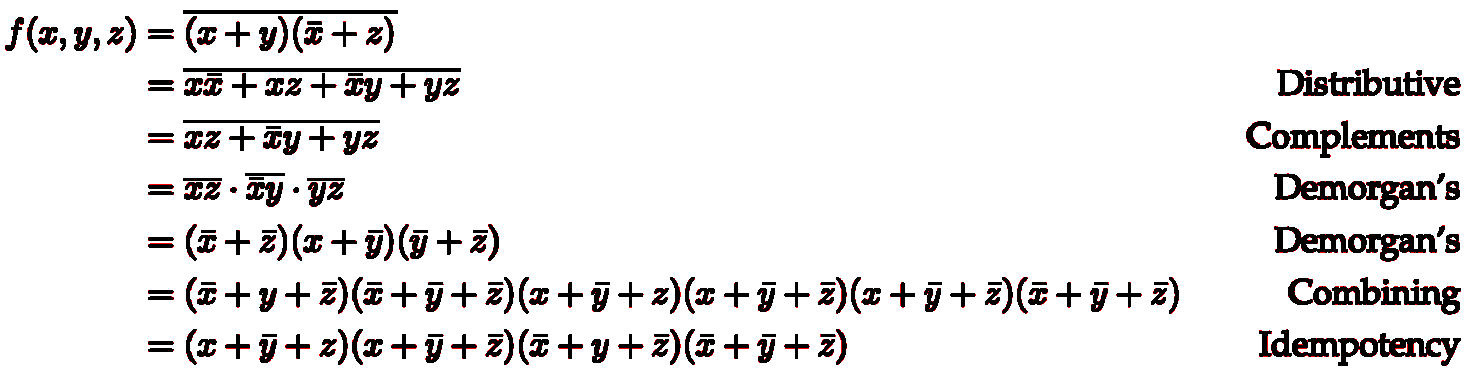
\includegraphics[width=0.8\columnwidth]{1.png}\\
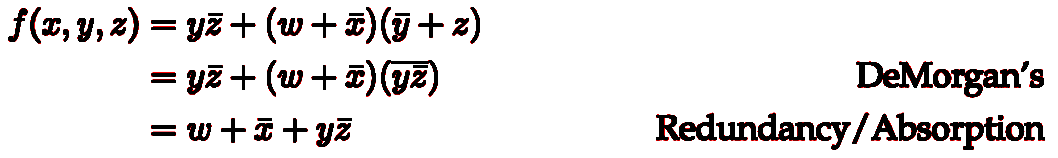
\includegraphics[width=0.56\columnwidth]{2.png}\\
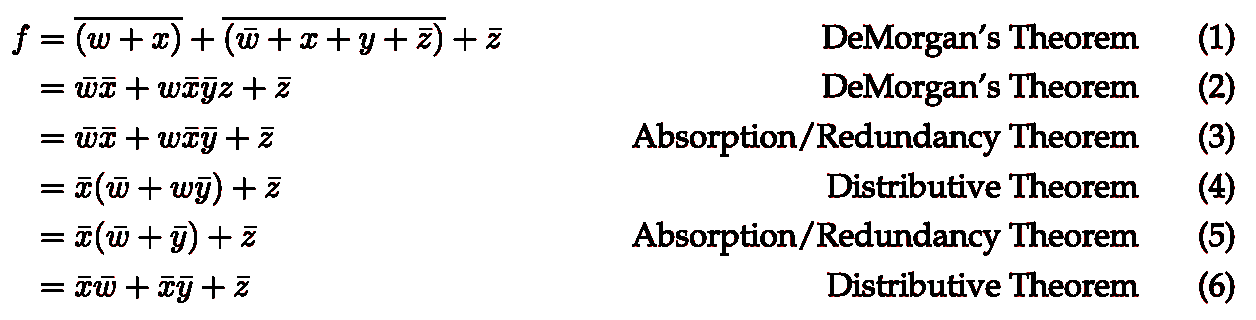
\includegraphics[width=0.7\columnwidth]{3.png}\\
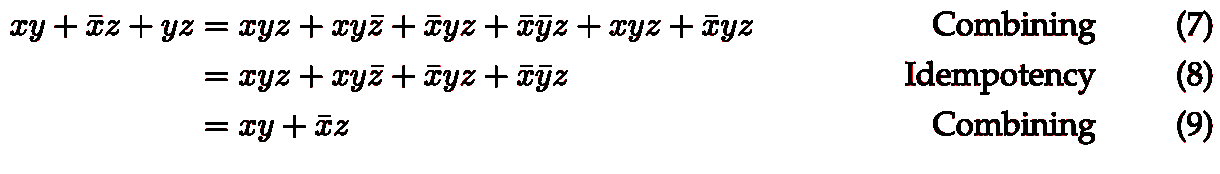
\includegraphics[width=0.7\columnwidth]{4.png}\\

\includegraphics[width=0.2\columnwidth]{markjeffrey-e1637952274628.jpg}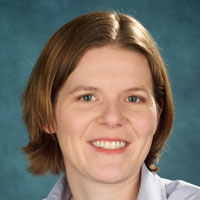
\includegraphics[width=0.2\columnwidth]{NatalieEnrightJerger.jpg}
\includegraphics[width=0.2\columnwidth]{markjeffrey-e1637952274628.jpg}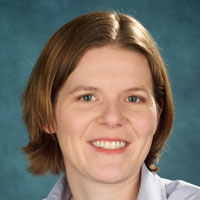
\includegraphics[width=0.2\columnwidth]{NatalieEnrightJerger.jpg}
\vspace{-6pt}
    \end{minipage}
};
%------------ PROPRIEDADES BOX ----------------
\node[fancytitle, right=10pt] at (box.north west) {Labs};
\end{tikzpicture}



%------------ CONTEÚDO COMANDOS DE TEXTO ---------------------
\begin{tikzpicture}
\node [mybox] (box){%
    \footnotesize\begin{minipage}{0.3\textwidth}
    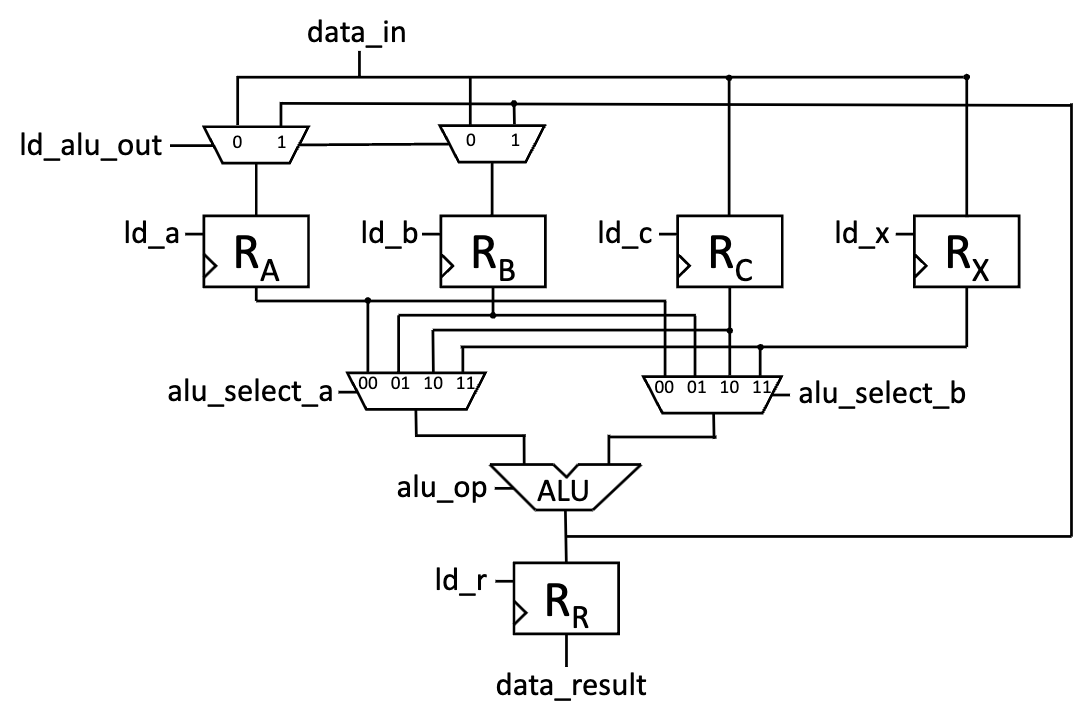
\includegraphics[width=0.7\columnwidth]{a.png} $Ax^2+Bx+C$
    \lstset{style=verilogStyle2}
\begin{lstlisting}
module FSM(input logic Clock, Reset, Go, input logic [7:0] DataIn, DataResult, output logic ResultValid);
    logic ld_a, ld_b, ld_c, ld_x, ld_r, ld_alu_out, alu_op;
    logic [1:0] alu_select_a, alu_select_b;
    control C0(...); // instantiate
    datapath D0(...);
endmodule

module control(
    input logic clk, reset, go, output logic ld_a, ..., ld_x, alu_op, ld_alu_out, result_valid, output logic [1:0] alu_select_a, alu_select_b);
    typedef enum logic [3:0]  {S_LOAD_A_RST='d0, ..., S_CYCLE_4='d13} statetype; // define states              
    statetype current_state, next_state;                            
    always_comb begin
        case (current_state)
            S_LOAD_A_RST: next_state = go ? S_LOAD_A_WAIT : S_LOAD_A_RST; 
            S_LOAD_A: next_state = go ? S_LOAD_A_WAIT : S_LOAD_A;
            S_LOAD_A_WAIT: next_state = go ? S_LOAD_A_WAIT : S_LOAD_B; 
            ...
            S_CYCLE_4: next_state = S_LOAD_A;
            default:   next_state = S_LOAD_A_RST;
        endcase end
    always_comb begin
        ld_alu_out = 1'b0;
        ... // make all signals 0
        result_valid = 1'b0;
        case (current_state)
            S_LOAD_A_RST: begin ld_a = 1'b1; end
            S_LOAD_A: begin ld_a = 1'b1; result_valid = 1'b1; end
            S_LOAD_B: begin ld_b = 1'b1; end
            ...
            S_CYCLE_4: begin // A*X*X + B*X + C
                ld_alu_out = 1'b0; 
                alu_select_a = 2'b00; 
                alu_select_b = 2'b01; 
                ld_r = 1'b1; end
        endcase end
    always_ff@(posedge clk) begin    // current_state logicisters
        if(reset) current_state <= S_LOAD_A_RST;
        else current_state <= next_state; end
endmodule

module datapath(...);
    logic [7:0] a, b, c, x, alu_out, alu_a, alu_b;
    always_ff @(posedge clk) begin
        if(reset) begin
            a <= 8'b0; ... // set all to 0
            x <= 8'b0; end
        else begin
            if(ld_a) a <= ld_alu_out ? alu_out : data_in; 
            if(ld_b) b <= ld_alu_out ? alu_out : data_in; 
            if(ld_c) c <= data_in;
            if(ld_x) x <= data_in; end end
    always@(posedge clk) begin // output logic result logicister
        if(reset) data_result <= 8'b0;
        elseif(ld_r) data_result <= alu_out; end
    always_comb begin
        case (alu_select_a)
            2'b00: alu_a = a; ... // set to whatever
            2'b11: alu_a = x;
            default: alu_a = 8'b0;
        endcase
        case (alu_select_b) endcase // same 
    end
    always_comb begin : ALU
        case (alu_op)
            0: alu_out = alu_a + alu_b; //performs addition
            1: alu_out = alu_a * alu_b; //performs multiplication
            default: alu_out = 8'b0;
        endcase end
endmodule
\end{lstlisting}
\vspace{-14pt}
    \end{minipage}
};
%------------ COMANDOS DE TEXTO BOX ---------------------
\node[fancytitle, right=10pt] at (box.north west) {Computer Organization};
\end{tikzpicture}




%------------ CONTEÚDO COMANDOS DE TEXTO ---------------------
\begin{tikzpicture}
\node [mybox] (box){%
    \footnotesize\begin{minipage}{0.3\textwidth}
    \lstset{style=assembly}
    Recursive findSum $\;\;\;\;\;\;\;\;\;\;\;\;\;\;\;\;\;\;\;$ Polling
    \vspace{-5pt}
\begin{lstlisting}
.data                           ...
N:          .word 5             _start: li s0, 0x... # addr of keys
.text                                   li s1, 0x... # addr of LEDRS
.global _start                  POLL:   lw s2, 0(s0)
_start:     la s4, N                    beqz s2, POLL # cont polling
            lw a0, 0(s4)        WAIT:   lw s3, 0(s0)
            jal FINDSUM                 bnez s3, WAIT # wait for release
END:        ebreak                      li s3, 1 # check for key0     
FINDSUM:    bnez a0, PUSH               andi s5, s2, 0x1 # mask presses
            jr ra (ra = EEE eventually) bne s5, s3, CHK_1
PUSH:       addi sp, sp, -8             li s4, 0 # value outputted
            sw a0, 4(sp)                j UPDATE
            sw ra, 0(sp)        CHK_1:  li s3, 2 #0b0010, key1
            addi a0, a0, -1             and s5, s2, s3
            jal FINDSUM                 bne s5, s3, CHK_2
EEE:        lw t0, 4(sp)                li s4, 1 # value outputted, s3-1
            add a0, a0, t0              j UPDATE 
            lw ra, 0(sp)        # for key2, key3, same for 0b0100, etc
            addi sp, sp, 8      UPDATE: sw s4, 0(s1) # lights up LED        
            jr ra                       j POLL
\end{lstlisting}
\vspace{-5pt}
Interrupts
\vspace{-5pt}
\begin{lstlisting}
.data
# Messages
msg_1: .asciz "Please take a deep breath" # msg_2, msg_3...
timeNow: .word 0xffff0018   # current time    
cmp: .word 0xffff0020       # time for new interrupt
display_ready_addr: 	.word 0xffff0008
display_register_addr:	.word 0xffff000c
.eqv OUT_CTRL 0xffff0008    # Display Related
.eqv OUT 0xffff000c
counter: .word 0
.text
main:   # Set time to trigger interrupt to be 5000 milliseconds
	la s0, cmp
	lw s0, 0(s0)
	li s1, 5000            # Stored Increment
	sw s1, 0(s0)           # Set timer value for interrupt
	addi s5, zero, 0       # Flag if interrupt has occurred 
	addi s2, zero, 4       # Case Out of bounds
	la t0, timer_handler   # Set the handler address and enable interrupts
	csrrw zero, utvec, t0  # Set utvec to handler address
	csrrsi zero, ustatus, 0x1 # Set interrupt enable bit
	csrrsi zero, uie, 0x10 # Set bit 4 to enable timer
	addi s9, zero, 1       # Case map. Start s9 at case 1
	addi s6, zero, 1
	addi s7, zero, 2
	addi, s8, zero, 3
LOOP:   beq s9, s6, SEND1
	beq s9, s7, SEND2
	beq s9, s8, SEND3
TICK:   jal PRINT
	addi s5, zero, 0       # Reset Flag
	addi s9, s9, 1         # Increment Case
	beq s9, s2, RESET_CASE # Case out of bounds
	j WAIT 
RESET_CASE:
	addi s9, zero, 1
	j WAIT
WAIT:   beqz s5, WAIT
	j LOOP
SEND1:  # Print Cases. SEND1, SEND 2... same
	la a0, msg_1
	j TICK
PRINT:  # Assumes a0 has the address of the msg
	addi t0, zero, 31      # Counter
	PRINT_LOOP:
	li t1, OUT  
	lb t2, 0(a0)
	sb t2, 0(t1)           # Sent to OUT
	addi a0, a0, 1         # Go to next byte
	addi, t0, t0, -1       # Decrement counter
	bnez t0, PRINT_LOOP    # Loop until 32 bytes have been printed
	jr ra
timer_handler:  addi sp, sp, -12   # Push registers to stack
	sw t0, 0(sp)
	sw t1, 4(sp)
	sw t2, 8(sp)
	la t0, cmp         # Update cmp and flag
	lw t0, 0(t0)       # t0 has the address of the time to compare to
	lw t1, 0(t0)       # t1 has the current time to compare to
	li t2, 5000
	add t1, t1, t2     # t1 has the old time to compare to + 5000
	sw t1, 0(t0)       # Update cmp
	addi s5, zero, 1   # Change flag to indicate interrupt has occurred
	lw t2, 8(sp)       # Pop Registers from stack
	lw t0, 4(sp)
	lw t1, 0(sp)
	addi sp, sp, 12
	uret
END: ebreak
\end{lstlisting}
% \begin{lstlisting}
% .global _start
% .text
% _start:
% 	la s2, LIST # Load the memory address into s2
% 	la s4, LIST # Same thing
% 	lw s3, 0(s2) # Store the length of the list in s3
% 	addi s4, s4, 4 # Address of first element of list
% 	addi s5, zero, 1 # Start with swapped = True
% 	j OUTER_LOOP
% OUTER_LOOP:
% 	addi s4, s2, 4
	
% 	addi s3, s3, -1 # One less than because we want to stop one place before the end
% 	add s6, zero, s3 # Copy s3 into s6 for inner loop
% 	beqz s5, END # If no swaps occurred, skip to end for efficiency
% 	beqz s3, END # If inner loop has run n times, it's over
% 	addi s5, zero, 0 # s5 is the "swapped flag"
% 	j INNER_LOOP
% INNER_LOOP:
% 	beqz s6 OUTER_LOOP
% 	add a0, zero, s4 
% 	jal SWAP
	
% 	# Check if swap occurred
% 	addi t3, zero, 1
% 	beq a0, t3, UPDATE_SWAPPED
% 	CONTINUE:	
% 		addi s4, s4, 4
% 		addi s6, s6, -1
% 		j INNER_LOOP
% SWAP:
% 	lw t0, 0(a0) # t0 stores the current element
% 	lw t1, 4(a0) # t1 stores the next element
% 	bge t0, t1, SWAP_FR
% 	addi a0, zero, 0
% 	jr ra
% SWAP_FR:
% 	sw t0, 4(a0) # Place the first element into the next spot in memory
% 	sw t1, 0(a0) # Place the second element into the current spot in memory
% 	addi a0, zero, 1
% 	jr ra
% UPDATE_SWAPPED:
% 	addi s5, zero, 1
% 	j CONTINUE
	
% END: ebreak
% .global LIST
% .data
% LIST:
% .word 10, 1400, 45, 23, 5, 3, 8, 17, 4, 20, 33
% \end{lstlisting}
\vspace{-14pt}
    \end{minipage}
};
%------------ COMANDOS DE TEXTO BOX ---------------------
\node[fancytitle, right=10pt] at (box.north west) {Assembly};
\end{tikzpicture}

\end{multicols*}
\end{document}
Contact GitHub API Training Shop Blog About
© 2016 GitHub, Inc. Terms Privacy Security Status Help